\documentclass[12pt]{report}
\usepackage[utf8]{inputenc}
\usepackage[russian]{babel}
%\usepackage[14pt]{extsizes}
\usepackage{listings}
\usepackage{graphicx}
\usepackage{amsmath,amsfonts,amssymb,amsthm,mathtools} 
\usepackage{pgfplots}
\usepackage{filecontents}
\usepackage{indentfirst}
\usepackage{eucal}
\usepackage{enumitem}
\frenchspacing

\usepackage{indentfirst} % Красная строка


\usetikzlibrary{datavisualization}
\usetikzlibrary{datavisualization.formats.functions}

\usepackage{amsmath}




% Для листинга кода:
\lstset{ %
language=haskell,                 % выбор языка для подсветки (здесь это С)
basicstyle=\small\sffamily, % размер и начертание шрифта для подсветки кода
numbers=left,               % где поставить нумерацию строк (слева\справа)
numberstyle=\tiny,           % размер шрифта для номеров строк
stepnumber=1,                   % размер шага между двумя номерами строк
numbersep=5pt,                % как далеко отстоят номера строк от подсвечиваемого кода
showspaces=false,            % показывать или нет пробелы специальными отступами
showstringspaces=false,      % показывать или нет пробелы в строках
showtabs=false,             % показывать или нет табуляцию в строках
frame=single,              % рисовать рамку вокруг кода
tabsize=2,                 % размер табуляции по умолчанию равен 2 пробелам
captionpos=t,              % позиция заголовка вверху [t] или внизу [b] 
breaklines=true,           % автоматически переносить строки (да\нет)
breakatwhitespace=false, % переносить строки только если есть пробел
escapeinside={\#*}{*)}   % если нужно добавить комментарии в коде
}

\usepackage[left=2cm,right=2cm, top=2cm,bottom=2cm,bindingoffset=0cm]{geometry}
% Для измененных титулов глав:
\usepackage{titlesec, blindtext, color} % подключаем нужные пакеты
\definecolor{gray75}{gray}{0.75} % определяем цвет
\newcommand{\hsp}{\hspace{20pt}} % длина линии в 20pt
% titleformat определяет стиль
\titleformat{\chapter}[hang]{\Huge\bfseries}{\thechapter\hsp\textcolor{gray75}{|}\hsp}{0pt}{\Huge\bfseries}


% plot
\usepackage{pgfplots}
\usepackage{filecontents}
\usetikzlibrary{datavisualization}
\usetikzlibrary{datavisualization.formats.functions}

\begin{document}
%\def\chaptername{} % убирает "Глава"
\thispagestyle{empty}
\begin{titlepage}
	\noindent \begin{minipage}{0.15\textwidth}
	
\includegraphics[width=\linewidth]{img/b_logo}
	\end{minipage}
	\noindent\begin{minipage}{0.9\textwidth}\centering
		\textbf{Министерство науки и высшего образования Российской Федерации}\\
		\textbf{Федеральное государственное бюджетное образовательное учреждение высшего образования}\\
		\textbf{~~~«Московский государственный технический университет имени Н.Э.~Баумана}\\
		\textbf{(национальный исследовательский университет)»}\\
		\textbf{(МГТУ им. Н.Э.~Баумана)}
	\end{minipage}
	
	\noindent\rule{18cm}{3pt}
	\newline\newline
	\noindent ФАКУЛЬТЕТ $\underline{\text{«Информатика и системы управления»}}$ \newline\newline
	\noindent КАФЕДРА $\underline{\text{«Программное обеспечение ЭВМ и информационные технологии»}}$\newline\newline\newline\newline\newline
	
	
	\begin{center}
		\noindent\begin{minipage}{1.3\textwidth}\centering
			\Large\textbf{  Отчет по лабораторной работе №3}\newline
			\textbf{по дисциплине "Операционные системы"}\newline\newline
		\end{minipage}
	\end{center}
	
	\noindent\textbf{Тема} $\underline{\text{Основы UNIX~~~~~~~~~~~~~~~~~~~}}$\newline\newline
	\noindent\textbf{Студент} $\underline{\text{Романов А.В.~~~~~~~~~~~~~~~}}$\newline\newline
	\noindent\textbf{Группа} $\underline{\text{ИУ7-53Б~~~~~~~~~~~~~~~~~~~~~~~}}$\newline\newline
	\noindent\textbf{Оценка (баллы)} $\underline{\text{~~~~~~~~~~~~~~~~~~~~~~}}$\newline\newline
	\noindent\textbf{Преподаватели} $\underline{\text{Рязанова Н.Ю.~~}}$\newline\newline\newline
	
	\begin{center}
		\vfill
		Москва~---~\the\year
		~г.
	\end{center}
\end{titlepage}

\newpage

\chapter{Задание №1}

Создаю папку IU7-53B с помощью команды mkdir, перемещаюсь в нее, с помощью команды cd, и создаю в ней папку Romanov. С помощью команды pwd вывожу полный путь до директории. Командой ls с различными флагами вывожу содержимое директории. 

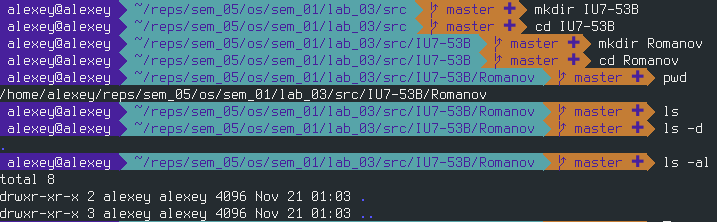
\includegraphics[width=\linewidth]{img/task01.png}

\chapter{Задание №2}

Запускаю команду ps -al до запуска программы, создающий дочерний процесс: 

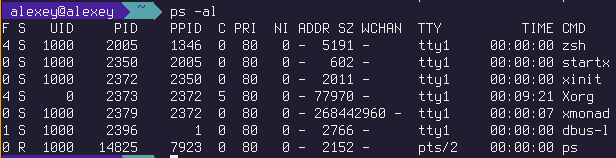
\includegraphics[width=\linewidth]{img/task02_01.png}

Запускаю команду ps -al после запуска программы, создающий дочерний процесс. Появляется два новых процесса с PID 14913 (родитель) и 14914 (потомок):

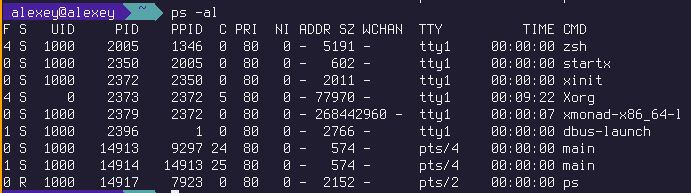
\includegraphics[width=\linewidth]{img/task02_02.png}

Удаляю с помощью команды kill потомка и убеждаюсь что процесс с PID 14914 теперь является процессом Зомби (Z):

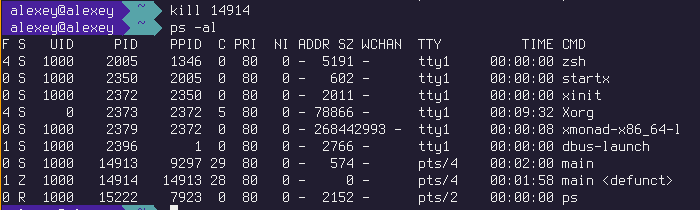
\includegraphics[width=\linewidth]{img/task02_04.png}

Перезапускаю программу и теперь удаляю родителя (PID 15335), получая процес сироту. Убеждаюсь, что процес сирота (PID 15336) усыновлен процессом с PID 1:

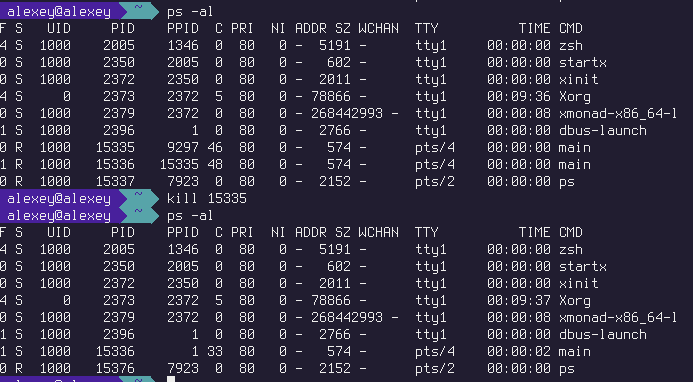
\includegraphics[width=\linewidth]{img/task02_05.png}

\chapter{Задание №3}

Создаю link на файл, и и с помощью команды ls -li убеждаюсь что и link и файл имеют одинаковый inode:

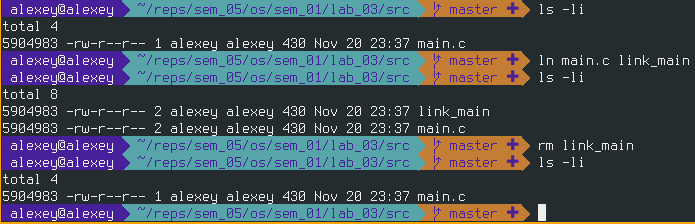
\includegraphics[width=\linewidth]{img/task03_01.png}

С помощью команды ln -sf создаю символическую ссылку на файл:

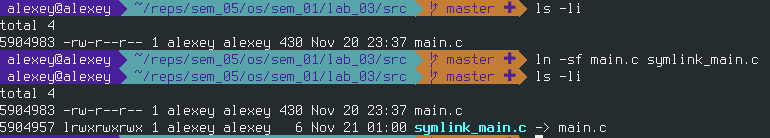
\includegraphics[width=\linewidth]{img/task03_02.png}

\chapter{Задание №4}

Создаю именованный программный канал командой mknod с именем pipe, и направляю текст в этот канал:

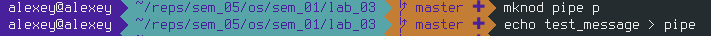
\includegraphics[width=\linewidth]{img/task04_01.png}


Открываю новый терминал и используя команду tee вывожу содержимое программного канала на экран:

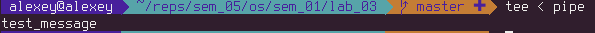
\includegraphics[width=\linewidth]{img/task04_02.png}

\bibliographystyle{utf8gost705u}  % стилевой файл для оформления по ГОСТу

\bibliography{51-biblio}          % имя библиографической базы (bib-файла)


\end{document}
